\documentclass[headings=optiontoheadandtoc,listof=totoc,parskip=full]{scrartcl}

\usepackage[tbtags]{amsmath,mathtools}
\usepackage{amsmath}
\usepackage{amssymb}
\usepackage{enumitem}
\usepackage[margin=.75in]{geometry}
\usepackage[headsepline]{scrlayer-scrpage}
\usepackage[USenglish]{babel}
\usepackage{hyperref}
\usepackage{graphicx}
\usepackage{float}
\usepackage{physics}
\usepackage[format=hang, justification=justified]{caption}
\usepackage{xcolor}
\usepackage{mathbbol}
\usepackage[backend=biber]{biblatex}
\usepackage{xurl}

\usepackage{cleveref} % Needs to be loaded last

\hypersetup{
	linktoc = all,
	pdfborder = {0 0 .5 [ 1 3 ]}
}
\captionsetup{width=.9\textwidth}
\addbibresource{citations.bib}

\def \reals {\mathbb{R}}
\DeclareMathOperator*{\argmax}{arg\,max}
\DeclarePairedDelimiter\floor{\lfloor}{\rfloor}

\pagestyle{scrheadings}
\rohead{Khedekar, Mangat \& Novotny}
\lohead{CS 479 Programming Assignment 3}

\title{Programming Assignment 3}
\subtitle{CS 479\\\url{https://github.com/alexander-novo/CS479-PA3}}
\author{Nikhil Khedekar\\33\%\\\Cref{sec:theory} \and Mehar Mangat\\33\%\\\Cref{sec:theory} \and Alexander Novotny\\33\%\\\Cref{sec:impl,sec:results}}
\date{Due: April 28, 2021 \\ Submitted: \today}

\begin{document}
\maketitle
\tableofcontents
\pagenumbering{gobble}

\newpage
\pagenumbering{arabic}

%%%%%%%%%%%%%%%%%%%%%%

\section{Theory}
\label{sec:theory}

This assignment explores the usage of Principal Component Analysis for dimensionality reduction in order to perform classifications on a dataset of provided images. The images were of faces from the FERET face database \cite{feretdataset}, and have a good variety of faces from different genders, ethnicity, age groups, lighting conditions, etc. The classification task to be performed was facial recognition

\subsection{Principal Component Analysis (PCA)}
\label{sec:theory-pca}
Principal Component Analysis (PCA) is a method for reducing the dimensionality of high dimensional data while preserving as much information as possible. The way this works is by the projection of the sample data along the principal distribution directions. Intuitively, this can be understood by finding the directions that capture the highest variance of the data and projecting the data along these directions. 


For some given sample data $\mathbf{X} = \{\mathbf{x}_i \in \reals^N, 1 \leq i \leq M\}$, where $M$ is the number of samples in the data set, the sample covariance matrix $\mathbf{\Sigma}_x$ can be found using \cref{eq:mean} and \cref{eq:cov_mat}, where $\mathbf{\Bar{x}}$ is the sample mean and $\Phi_i$ are the normalized data points:
%
\begin{align} 
    \mathbf{\Bar{x}} &= \frac{1}{M}\sum_{i = 1}^{M}\mathbf{x}_i \label{eq:mean}\\
    \mathbf{\Phi_i} &= \mathbf{x}_i - \mathbf{\Bar{x}}\\
    \mathbf{\Sigma_x} &= \frac{1}{M}\sum_{i = 1}^M(\mathbf{x} - \mathbf{\Bar{x}})(\mathbf{x} - \mathbf{\Bar{x}})^\top \nonumber\\
        &= \frac{1}{M}\sum_{i = 1}^{M}\mathbf{\Phi}_i\mathbf{\Phi}_i^\top \label{eq:cov_mat}
\end{align}
%
\Cref{eq:cov_mat} can be further simplified to \cref{eq:cov_mat_simp} using \cref{eq:a_mat}.
%
\begin{align}
    \mathbf{\Sigma_x} &= \frac{1}{M}\mathbf{A}\mathbf{A}^\top, \label{eq:cov_mat_simp}\\
    \intertext{where}
    \mathbf{A} &= [\Phi_1 \Phi_2 ... \Phi_M] \label{eq:a_mat}
\end{align}
%
The eigenvectors and eigenvalues of the covariance matrix $\mathbf{\Sigma}_x$ have the special property that the eigenvectors form an orthogonal basis in $\reals^N$ for the sample data with the corresponding eigenvalues representing the variance of the data in these directions. The eigenvectors $\mathbf{u}_i$ and corresponding eigenvalues $\lambda_i$ are obtained using \cref{eq:eigenvec_and_eigenval}.
%
\begin{equation}\label{eq:eigenvec_and_eigenval}
    \mathbf{\Sigma_x}\mathbf{u_i} = \lambda_i\mathbf{u}_i
\end{equation}
%
However, in image recognition this approach becomes problematic. Performing PCA directly on the image's covariance matrix can be computationally intractable. Even considering small images of $50 \times 50$ pixels, the covariance matrix would contain $2500$ elements!

Fortunately though, there is a workaround. The rank of the covariance matrix is limited by the number of images in our data-set. So, if the number of images in our data-set is smaller than the number of dimensions of the image, then we can perform the following calculation:

Let $\mathbf{A}$ be a matrix of the images, where each column contains a mean-subtracted image from the data-set. Then the eigenvector decomposition of the covariance matrix $\mathbf{\Sigma}_x$  can be computed as:

\begin{equation}\label{eq:eigen_vector_aaT}
    \mathbf{\Sigma}_x\mathbf{u}_i = \mathbf{AA}^\top \mathbf{u}_i = \lambda_i\mathbf{u}_i
\end{equation}

However, we can multiply $\mathbf{A}$ to \cref{eq:eigen_vector_aaT}, to get:

\begin{equation}\label{eq:eigen_vector_aaaT}
\mathbf{A^\top AA^\top} \mathbf{u}_i = \lambda_i \mathbf{A}^\top \mathbf{u}_i
\end{equation}

Using the definition in \cref{eq:eigenvector_rewrite} in \cref{eq:eigen_vector_aaaT}, we can see that $\mathbf{v}_i$ represents the eigenvector for $\mathbf{A^\top A}$. 

\begin{equation}\label{eq:eigenvector_rewrite}
    \mathbf{v}_i = \mathbf{A}^\top \mathbf{u}_i
\end{equation}


% then we can multiply both sides of the equation by $\mathbf{A}$ to obtain:

% \begin{equation}
% \mathbf{AA}^\top u_i = \lambda_i \mathbf A u_i
% \end{equation}

% This means that if $u_i$ is an eigenvector of $\mathbf{A^\top A}$, then the eigenvector from $\mathbf{AA^\top}$ must be a a multiple of $u_i$ - that is:

% \begin{equation}
%     v_i = \mathbf Au_i
% \end{equation}

This drastically reduces the necessary size of the covariance matrix. If we had 75 images that were $50 \times 50$ before, then the matrix $\mathbf{A^\top A}$ is $75 \times 75$, which is much more reasonable to calculate than a $2500 \times 2500$ covariance matrix.

\subsection{Mahalanobis Distance}
\label{sec:theory-mahalanobis}

The Mahalanobis Distance $e_k$ between two vectors, $\mathbf{x}$ and $\mathbf{y}$, projected onto the span of the chosen eigenvectors is given by \cref{eq:mahalanobis}.

\begin{equation}
    e_k^2 = \sum_{j=1}^K \frac{1}{\lambda_j} (x_j - y_j) \label{eq:mahalanobis}
\end{equation}

The advantage Mahalanobis distance has over Euclidean is two-fold in this experiment; Mahalanobis distance accounts for the correlations between variables, and is also scale invariant. The scale in-variance is crucial as it saves us a step in normalization that Euclidean distance would otherwise incorrectly capture.


\subsection{Application}
\label{sec:theory-application}
In our notation, we assume that the eigenvalues are indexed in descending order, namely, $\lambda_1 > \lambda_2 > ... > \lambda_N$. Using the eigenvectors as the new basis for our data we can represent our data samples $\mathbf{x} \in \reals^N$ by \cref{eq:eigenvec_rep}

\begin{equation}\label{eq:eigenvec_rep}
    \mathbf{x} - \mathbf{\Bar{x}} = \sum_{i = 1}^N y_i\mathbf{u}_i = y_1\mathbf{u}_1 + y_2\mathbf{u}_2 + ... y_N\mathbf{u}_N
\end{equation}

where $y_1, y_2 ... y_N$ are the coefficients in this new basis and are given by \cref{eq:yi}.

\begin{equation}\label{eq:yi}
    y_i = \frac{(\mathbf{x} - \mathbf{\Bar{x}})^\top \mathbf{u}_i}{\mathbf{u}_i\mathbf{u}_i^\top} = (\mathbf{x} - \mathbf{\Bar{x}})^\top\mathbf{\hat{u}}_i
\end{equation}

where $\mathbf{\hat{u}}_i$ represents the unit vector in the direction of $\mathbf{u}_i$. The final dimensionality reduction is carried out on the basis of \cref{eq:eigenvec_rep} in that only the components corresponding to the first $K (K << N)$ eigenvectors are kept and the remaining components are discarded. This formulation approximates $\mathbf{x}$ by $\mathbf{\hat{x}}$ for which \cref{eq:eigenvec_rep} can be rewritten as \cref{eq:eigenvec_rep_pc}.

\begin{equation}\label{eq:eigenvec_rep_pc}
    \mathbf{\hat{x}} - \mathbf{\Bar{x}} = \sum_{i = 1}^N y_i\mathbf{u}_i = y_1\mathbf{u}_1 + y_2\mathbf{u}_2 + ... y_K\mathbf{u}_K
\end{equation}

\cref{eq:eigenvec_rep_pc} can be written in matrix form instead of the summation as \cref{eq:linear_transform_1}

\begin{equation}\label{eq:linear_transform_1}
    \mathbf{\hat{x}} - \mathbf{\Bar{x}} = \mathbf{U}\begin{bmatrix}y_1\\y_2\\...\\y_K\end{bmatrix}
\end{equation}

where $\mathbf{U} = [\mathbf{u}_1, \mathbf{u}_2, ... , \mathbf{u}_K]$ is an $N \times K$ matrix with its columns as the $K$ largest eigenvectors of the covariance matrix $\mathbf{\Sigma}_x$. \Cref{eq:linear_transform_1} can also be written as 

\begin{equation}\label{eq:linear_transform_2}
    \begin{bmatrix}y_1\\y_2\\...\\y_K\end{bmatrix} = \mathbf{U}^\top(\mathbf{\hat{x}} - \mathbf{\Bar{x}})
\end{equation}

The choice of $K$ is made on the basis of the amount of information that we wish to preserve. For a numerical representation of the information preserved, we can specify a threshold $t$ for the ratio of the summations of the first $K$ eigenvalues to that of all $N$ eigenvalues as \cref{eq:thresholding}. A threshold of 1 would mean perfect information retention (and consequently, no reduction in dimensionality).

\begin{equation}\label{eq:thresholding}
    \frac{\sum_{i = 1}^K\lambda_i}{\sum_{i = 1}^N\lambda_i} > t
\end{equation}

Finding these components $y_i$ have several applications, one of which is the subject of this assignment. These components can be used to simplify the problem of comparing high dimensional data as is discussed in the next section.

\subsection{Eigenfaces and Facial Recognition}
\label{sec:theory-eigenfaces}

The first widely successful method of solving the facial recognition problem is the eigenface method \cite{eigenfaces}. The core of this method relies on the fact that image data can be stacked to form vectors in a dataset after which we can use PCA to reduce the dimensionality of the data and find the components $y_i$ described in the previous section. Similarity in the components implies a similarity in the data provided that the amount of information that is kept (decided using the threshold $t$) is enough for doing so. As the eigenvectors obtained by this method are essentially images themselves and given that the method was designed for recognizing images of faces, they are termed as eigenfaces. In dealing with images of faces, the mean vector $\mathbf{\Bar{x}}$ is also now termed as the mean face. Hence, \cref{eq:eigenvec_rep} for image data would semantically represent the difference between a sample image and the mean face being given by a summation of the eigenfaces scaled by their respective components. 

Facial recognition intends to solve the problem of finding an image in a given dataset that is visually the most similar to a test image. The comparison of images is a computationally heavy task as it has the complexity of $\mathcal O(rc)$ where $r, c$ are the rows and columns of the image respectively. The complexity of this task can be reduced to $\mathcal O(K)$ by finding the eigenfaces and scalar components that represent each image and reducing it to $K$ components. This is essentially an application of PCA.

\section{Implementation}
\label{sec:impl}
Similarly to previous assignments, the Eigen~\autocite{eigen} C++ template library was used to handle matrix operations. The C++ standard \texttt{filesystem} library~\autocite{filesystem} new to C++17 was also used for reading in the contents of an entire directory for reading in the data set. Many trivially parallelizable sections were parallelized using OpenMP, and all of Eigen's trivially parallelizable algorithms are already parallelized using OpenMP.

The training portion of the program begins by reading all of the training images into a large $M \times N$ Eigen matrix, where $M$ is the number of pixels in each image and $N$ is the number of images. We load the directory contents and the header of a single image to determine the size of the matrix before reading in the images so that reading may be done in parallel. Then, the mean is calculated using a standard parallel sum. Eigen helpfully includes a ``broadcasting'' module \autocite{eigenBroadcast} which lets us apply a vector operation to an entire matrix in a similar way to ``broadcasting'' that vector as a full matrix but without allocating an entire matrix. This is used to calculate $\mathbf A$ in \cref{eq:a_mat} by broadcasting the operation of subtracting the mean from the matrix of images. Then, Eigen's \texttt{SelfAdjointEigenSolver}~\autocite{eigenSolver} library is used to efficiently compute the eigenvalues and eigenvectors of $\mathbf{A^\top A}$ as discussed in \cref{sec:theory-pca}, which are already normalized and sorted in ascending order. 

According to Eigen's documentation, taking advantage of the symmetric nature of $\mathbf{A^\top A}$ gives us a speed increase of about 3 times that of a normal eigensolver. Additionally, as discussed in \cref{sec:theory}, $\mathbf{A^\top A}$ may be smaller than $\mathbf{AA}^\top$ - and in the case of the high resolution images, there are about 1000 images with about 2000 pixels each, so due to the cubic nature of the eigensolver algorithm, the use of the smaller $\mathbf{A^\top A}$ gives us another speed increase of about 8 times. Multiplying by $\mathbf A$ to obtain eigenvectors of $\mathbf{AA}^\top$ may denormalize the eigenvectors, so Eigen's broadcasting module is used again to normalize them (obtaining $\mathbf U$ ) and project the images onto the calculated eigenvectors by multiplying by $\mathbf A$ as in \cref{eq:linear_transform_2} (knowing that the columns of $\mathbf A$ are the mean subtracted from each image). The mean image, eigenvalues, projected images, and their labels are then written to a training data file to be read by the second portion of the program.

The testing portion of the program begins by reading all of the testing images into a matrix in a similar fashion to the training portion as well as the training data generated by said portion. Then, $K$ is calculated as in \cref{eq:thresholding} based on the inputted $t$. The test images are projected in the same way as the training images were, however this time only using the right $K$ columns of $\mathbf U$ to project (using Eigen's block operations module \autocite{eigenBlock}). Then the Mahalanobis distance is calculated between each projected testing and training images (taking care to only use the bottom $K$ rows of the projected training image matrix with Eigen's block module) as described in \cref{eq:mahalanobis}, ignoring the extra square as the square function is strictly increasing and doesn't affect comparisons. Each projected testing image uses a max heap to keep the running minimum 50 distances as it calculates every distance. Then this heap is sorted and checked for correct matches to classify. These distances and heap calculations are trivially parallelizable for each projected testing image, so OpenMP is used to do it quickly.

\section{Results and Discussion}
\label{sec:results}

The calculated sample mean images for both data set can be found in \cref{fig:sample-means}. Note the appearance of a single pixel-wide border of dark pixels around both means - this seems to come from some sort of artifact in the original data sets consisting of slightly darker pixels on the border.

\begin{figure}[H]
	\centering
	\includegraphics[width=.2\textwidth]{../out/mean-H} \qquad
	\includegraphics[width=.2\textwidth]{../out/mean-L}
	\caption{The sample mean face for the high resolution data set (left) and the low resolution data set (right).}
	\label{fig:sample-means}
\end{figure}

The 10 largest and smallest eigenfaces can be found in \cref{fig:largest-eigen-H,fig:largest-eigen-L}. Note that the largest eigenfaces all look like faces in some way, while the smallest eigenfaces might as well be random noise. This is a good justification for dimensionality reduction using PCA - these smallest eigenfaces are contributing very little meaningful data. Also note that each eigenface calculated from the low resolution data corresponds to one calculated from the high resolution data almost exactly. This makes sense, since the low resolution images are just sampled version of the high resolution images, so it would make sense that the principal components are just sampled version of the principle components of the high resolution images. It also implies that principle components persist through downsampling. Note that eigenfaces 7 and 8 correspond but are inverted between data sets - this is an example of how inverted eigenvectors are still eigenvectors. Finally, note how many of the eigenfaces look seemingly male - this is probably due to the over-representation of male-presenting subjects in the data set.

\begin{figure}[H]
	\centering
	\includegraphics[width=.09\textwidth]{../out/eigenface-H-largest-1}
	\includegraphics[width=.09\textwidth]{../out/eigenface-H-largest-2}
	\includegraphics[width=.09\textwidth]{../out/eigenface-H-largest-3}
	\includegraphics[width=.09\textwidth]{../out/eigenface-H-largest-4}
	\includegraphics[width=.09\textwidth]{../out/eigenface-H-largest-5}
	\includegraphics[width=.09\textwidth]{../out/eigenface-H-largest-6}
	\includegraphics[width=.09\textwidth]{../out/eigenface-H-largest-7}
	\includegraphics[width=.09\textwidth]{../out/eigenface-H-largest-8}
	\includegraphics[width=.09\textwidth]{../out/eigenface-H-largest-9}
	\includegraphics[width=.09\textwidth]{../out/eigenface-H-largest-10}\\
	\includegraphics[width=.09\textwidth]{../out/eigenface-H-smallest-1}
	\includegraphics[width=.09\textwidth]{../out/eigenface-H-smallest-2}
	\includegraphics[width=.09\textwidth]{../out/eigenface-H-smallest-3}
	\includegraphics[width=.09\textwidth]{../out/eigenface-H-smallest-4}
	\includegraphics[width=.09\textwidth]{../out/eigenface-H-smallest-5}
	\includegraphics[width=.09\textwidth]{../out/eigenface-H-smallest-6}
	\includegraphics[width=.09\textwidth]{../out/eigenface-H-smallest-7}
	\includegraphics[width=.09\textwidth]{../out/eigenface-H-smallest-8}
	\includegraphics[width=.09\textwidth]{../out/eigenface-H-smallest-9}
	\includegraphics[width=.09\textwidth]{../out/eigenface-H-smallest-10}
	\caption{The 10 largest eigenfaces in decreasing order for the high resolution data set, followed by the 10 smallest eigenfaces in increasing order.}
	\label{fig:largest-eigen-H}
\end{figure}

\begin{figure}[H]
	\centering
	\includegraphics[width=.09\textwidth]{../out/eigenface-L-largest-1}
	\includegraphics[width=.09\textwidth]{../out/eigenface-L-largest-2}
	\includegraphics[width=.09\textwidth]{../out/eigenface-L-largest-3}
	\includegraphics[width=.09\textwidth]{../out/eigenface-L-largest-4}
	\includegraphics[width=.09\textwidth]{../out/eigenface-L-largest-5}
	\includegraphics[width=.09\textwidth]{../out/eigenface-L-largest-6}
	\includegraphics[width=.09\textwidth]{../out/eigenface-L-largest-7}
	\includegraphics[width=.09\textwidth]{../out/eigenface-L-largest-8}
	\includegraphics[width=.09\textwidth]{../out/eigenface-L-largest-9}
	\includegraphics[width=.09\textwidth]{../out/eigenface-L-largest-10}\\
	\includegraphics[width=.09\textwidth]{../out/eigenface-L-smallest-1}
	\includegraphics[width=.09\textwidth]{../out/eigenface-L-smallest-2}
	\includegraphics[width=.09\textwidth]{../out/eigenface-L-smallest-3}
	\includegraphics[width=.09\textwidth]{../out/eigenface-L-smallest-4}
	\includegraphics[width=.09\textwidth]{../out/eigenface-L-smallest-5}
	\includegraphics[width=.09\textwidth]{../out/eigenface-L-smallest-6}
	\includegraphics[width=.09\textwidth]{../out/eigenface-L-smallest-7}
	\includegraphics[width=.09\textwidth]{../out/eigenface-L-smallest-8}
	\includegraphics[width=.09\textwidth]{../out/eigenface-L-smallest-9}
	\includegraphics[width=.09\textwidth]{../out/eigenface-L-smallest-10}
	\caption{The same figure as \cref{fig:largest-eigen-H}, but for the low resolution data set.}
	\label{fig:largest-eigen-L}
\end{figure}

A comparison of classification accuracies between data sets can be found in \cref{fig:classification-accuracy}. There are a couple of interesting points to be found in the high resolution data set: while the 95\% information classifier starts as the most performant classifier (for $N = 1$), it is quickly surpassed by the other classifiers, becoming the least performing classifier at $N = 50$. Also, while the 80\% classifier starts as the least performant classifier, it is at times the most performant and eventually always at least matches the performance of the other classifiers. The low resolution classifiers, however, do not demonstrate this quality - the lower information classifiers remain lower performing. This face, along with the fact that the most performant low resolution classifiers at either end of the spectrum outperform the high resolution classifiers leads us to believe that the dimensionality of the data is still too large after performing PCA on the high resolution images, while the low resolution images benefit from low dimensionality data from the beginning. Despite this, the plots suggest that lowering the amount of information preserved by PCA for the high resolution images would only decrease the performance for $N = 1$ (even if it could recover performance for larger $N$), supporting our theory from above that downsampling, at times, may outperform PCA. A final interesting point is while there seems to be little improvement to be made on these classifiers for large $N$, there may be some room for improvement for $N = 1$. Note that the gaps between accuracies at $N = 1$ shrink as we increase the amount of data, and in the high resolution data set, the gap between 90\% and 95\% information is almost nonexistent, implying that preserving more information will not improve the accuracy. Meanwhile, the gap between 90\% and 95\% information in the low resolution data set is still quite large, implying there is some room for improvement by preserving more information - even though it already performs better than the high resolution data set at only 95\%.

\begin{figure}[H]
	\centering
	\includegraphics[width=\textwidth]{../out/compare-80-90-95}
	\caption{A comparison of classification accuracy against number of images considered ($N$), the percentage of information preserved by eigenfaces, and the data set used. The most performant classifier at each end of the spectrum of $N$ is marked in red for each data set.}
	\label{fig:classification-accuracy}
\end{figure}

A selection of faces matched with the faces they were classified as are available in \cref{fig:classifications-H,fig:classifications-L}. Something interesting to note is that these selections of images were chosen arbitrarily, and yet two of the three incorrectly classified images seem to be of either female or female-presenting subjects, and the images they were matched against depict similarly female or female-presenting subjects - all despite female-presenting subjects making up a relatively smaller number of subjects in the data set than male-presenting subjects. This is probably the reason - as explained above, PCA picked the principle components of male faces due to their over-representation, and now struggles to classify female faces which probably project weaker onto the span of male principle components. However, since all images of female-presenting subjects project weaker onto this span, they are relatively closer together than all of the images depicting male-presenting subjects, so PCA is still able to tell that they depict female-presenting subjects. This partially persists through to the low resolution images, where this time only one of the incorrectly classified images is female (incorrect image number 2). However, it is still matched to the downsampled version of the same image its high resolution version was matched to. This suggests that the difference between male-presenting and female-presenting face largely persist through downsampling, but some features become unrecognizable.

\begin{figure}[H]
	\centering
	\includegraphics[width=.15\textwidth]{../Images/fb_H/01001_960627_fb}
	\includegraphics[width=.15\textwidth]{../Images/fb_H/00261_940128_fb}
	\includegraphics[width=.15\textwidth]{../Images/fb_H/00863_940307_fb}
	\quad
	\includegraphics[width=.15\textwidth]{../Images/fb_H/00556_940519_fb}
	\includegraphics[width=.15\textwidth]{../Images/fb_H/00212_940128_fb_a}
	\includegraphics[width=.15\textwidth]{../Images/fb_H/00695_941121_fb}\\
	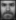
\includegraphics[width=.15\textwidth]{../Images/fa_H/01001_960627_fa}
	\includegraphics[width=.15\textwidth]{../Images/fa_H/00261_940128_fa}
	\includegraphics[width=.15\textwidth]{../Images/fa_H/00863_940307_fa}
	\quad
	\includegraphics[width=.15\textwidth]{../Images/fa_H/00557_940519_fa}
	\includegraphics[width=.15\textwidth]{../Images/fa_H/00266_940128_fa}
	\includegraphics[width=.15\textwidth]{../Images/fa_H/01005_960627_fa}
	\caption{High resolution testing images (top) and the training images they were matched against (bottom). Images which were correctly classified (i.e. both pictures are of the same subject) on the left, and incorrect classifications on the right.}
	\label{fig:classifications-H}
\end{figure}

\begin{figure}[H]
	\centering
	\includegraphics[width=.15\textwidth]{../Images/fb_L/01001_960627_fb}
	\includegraphics[width=.15\textwidth]{../Images/fb_L/00261_940128_fb}
	\includegraphics[width=.15\textwidth]{../Images/fb_L/00863_940307_fb}
	\quad
	\includegraphics[width=.15\textwidth]{../Images/fb_L/00770_960530_fb_a}
	\includegraphics[width=.15\textwidth]{../Images/fb_L/00212_940128_fb_a}
	\includegraphics[width=.15\textwidth]{../Images/fb_L/00695_941121_fb}\\
	\includegraphics[width=.15\textwidth]{../Images/fa_L/01001_960627_fa}
	\includegraphics[width=.15\textwidth]{../Images/fa_L/00261_940128_fa}
	\includegraphics[width=.15\textwidth]{../Images/fa_L/00863_940307_fa}
	\quad
	\includegraphics[width=.15\textwidth]{../Images/fa_L/00494_940519_fa}
	\includegraphics[width=.15\textwidth]{../Images/fa_L/00266_940128_fa}
	\includegraphics[width=.15\textwidth]{../Images/fa_L/00968_960627_fa}
	\caption{The same figure as \cref{fig:classifications-H}, but with images from the low resolution data set.}
	\label{fig:classifications-L}
\end{figure}

The ROC curve depicted in \cref{fig:intruders} allows us to compare the high/low resolution classifiers when applied to intruder detection. It seems that, like above, the low resolution classifier outperforms the high resolution classifier (as it has reduced area above the curve).

\begin{figure}[H]
    \centering
    \includegraphics[width=.75\textwidth]{../out/intruders}
    \caption{A comparison of intruder-detection ROC curves based on resolution.}
    \label{fig:intruders}
\end{figure}

\printbibliography

\end{document}